\documentclass[hyperref={pdfpagelabels=false}]{beamer}
\usepackage{lmodern}
\usepackage{amsmath}
\usepackage{graphicx}
\title{Explaining and Forecasting Online Auction
Prices and Their Dynamics Using
Functional Data Analysis}   
\author{Christopher Thiemann genannt Trappmann} 
\date{January 29, 2019} 
\beamertemplatenavigationsymbolsempty

\setbeamercolor{footline}{fg=blue}
\setbeamerfont{footline}{series=\bfseries}

\addtobeamertemplate{navigation symbols}{}{%
    \usebeamerfont{footline}%
    \usebeamercolor[fg]{footline}%
    \hspace{1em}%
    \insertframenumber/\inserttotalframenumber
}

\begin{document}

\begin{frame}
\titlepage
\end{frame}

\begin{frame}{Introduction} %feel free to ask questions ?
\begin{itemize}
	\item Why did I choose the paper? %"Interested in how to apply the methods we leanred here, some background in auction theory here in my bachelöors"
	\item Here focus on the (functional) methods beeing used.
\end{itemize}
\end{frame}

\begin{frame}{Overview}
\begin{itemize}
	\item Why auctions? %"name some applications" auctions pupular %name examples
	\item Why dynamic functional forcasting model?
	\begin{itemize}
		\item deal with unevenly spaced observations
		\item capture price dynamics
	\end{itemize}	
\end{itemize}
overall structure of the paper
\begin{itemize}
	\item use Functional regression to explore price evolution and velocity
	\item use results to build the forecasting model
\end{itemize}
\end{frame}

\begin{frame}{Auction Framework}
\begin{itemize}
	\item ebay
	\item second price sealed bid with proxy bidding
\end{itemize}
Data
\begin{itemize}
	\item 7 Day Auctions
	\item Microsoft Xbox and Harry Potter and the half blood prince
	\item Responds Variable: Bid History
\end{itemize}
\end{frame}

\begin{frame}{Bid-History} %erklärend bid spacing usw.
\begin{minipage}[c]{0.65\textwidth}
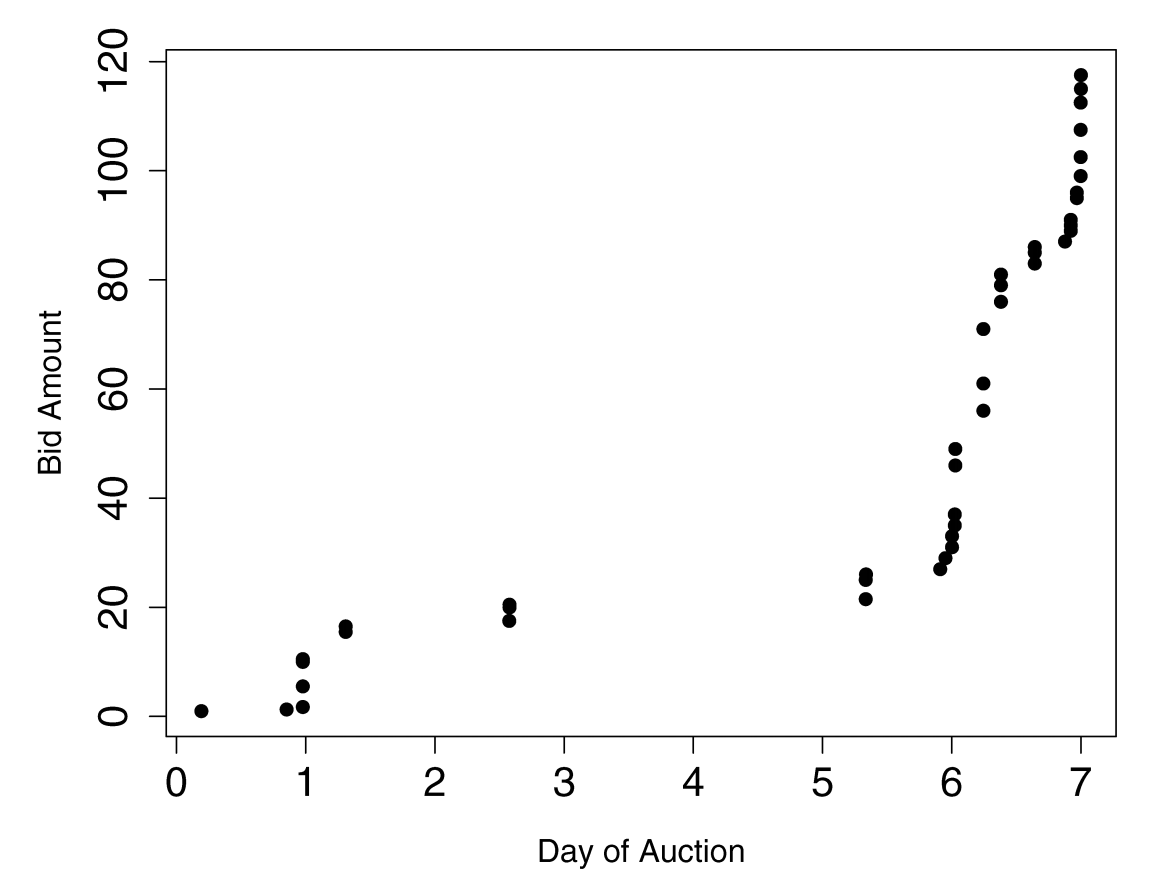
\includegraphics[width=\textwidth]{Auction_cleaned_scatter.pdf}
\end{minipage}
\hfill
\begin{minipage}[c]{0.3\textwidth}
\begin{itemize}
\item unevenly spaced observations
\item sparse in the middle
\item dense at the begining and end
\item bidsniping
\end{itemize}
\end{minipage}
\end{frame}

\begin{frame}{Auction Framework} %maybe not completelyy trivial if for examplke second highest bid bnelow reserve price
\begin{itemize}
	\item ebay
	\item second price sealed bid with proxy bidding
\end{itemize}
Data
\begin{itemize}
	\item 7 Day Auctions
	\item Microsoft Xbox and Harry Potter and the half blood prince
	\item Responds Variable: Bid History
	\item Explanatory variables: opening bid, final price, number of bids, seller rating, bidder rating, reserve price, condition, early bidding, jump bidding
\end{itemize}
\end{frame}

\begin{frame}{Functional Regression}
\begin{itemize}
	\item use FR to explore price dynamics
	\item relate functional responds variable to scalar covariates
	\item Modeltype: $\mathbf{y}(t)=\mathbf{X}^T\beta(t)+\mathbf{\epsilon}(t)$ %put emphasise on y(t) in comparison to the lecturre weher it was a scalar ,,,,,explain notation fett y ids vector of functions but i will talk about it in more detail later, if we plug in y'(t) we can model price velocity, critic no assumption on epsiloin?
	\item before however: recover functional data
\end{itemize}
\end{frame}

\begin{frame}{Irregular spacing of bids 1/3}
\centering
\begin{minipage}[c]{0.6\textwidth}
\includegraphics[width=\textwidth]{Auction1}
\end{minipage}
%\hfill
\begin{minipage}[c]{0.6\textwidth}
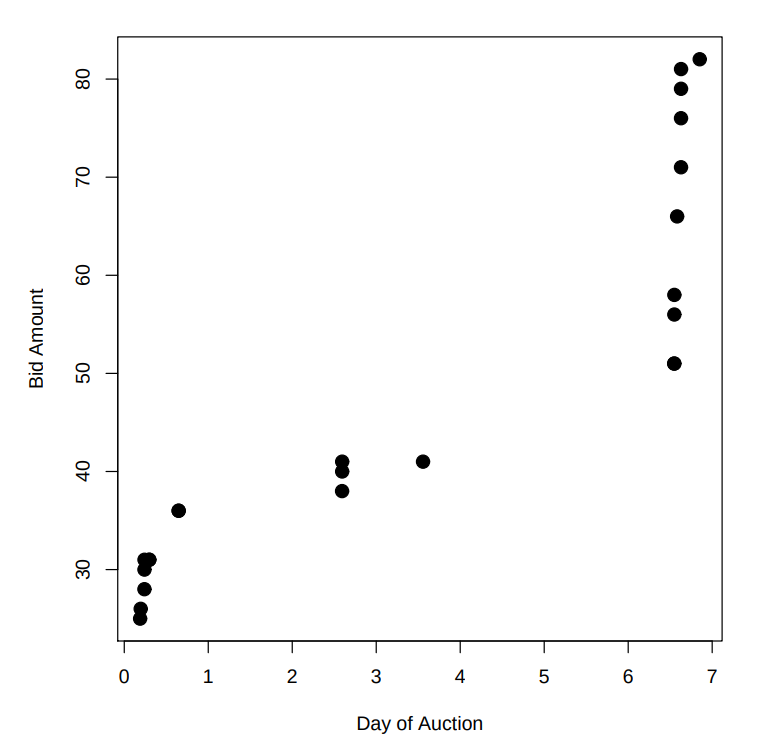
\includegraphics[width=\textwidth]{Auction2}
\end{minipage}
\end{frame}

\begin{frame}{Irregular spacing of bids 2/3}
\begin{minipage}[c]{0.65\textwidth}
\includegraphics[width=\textwidth]{log_int.pdf}
\end{minipage}
\hfill
\begin{minipage}[c]{0.3\textwidth}
\begin{itemize}
\item log bids
\item linear interpolate
\item sampling from common grid
\item bidsniping
\end{itemize}
\end{minipage} 
\end{frame}

\begin{frame}{Irregular spacing of bids 3/3}
%bild aus denenn von oben an einem common point gezogen wurde wie legt man diese puunkte ?? 
\end{frame}

\begin{frame}{Penalized smoothing spline}
\begin{align*}
\mathbf{y}^{(j)}=(y_1^{(j)},...,y_n^{(j)}) \ \ \ \ \ \	 j=1,...,N 
\end{align*}
 %"representation of each auction" 

polynomial spline %kjurzes bild an der tafel machen
\begin{align*}
f(t)=\beta_0+\beta_2t+\beta_2t^2+...+\sum_{l=q}^L \beta_{pl}(t-\tau_l)^p_+ \\ 
\end{align*}
penalized smoothing spline
\begin{align*}
PENN^{(j)}_{\lambda,m}=\sum_{i=1}^n (y_i^{(j)}-f^{(j)}(t_i))^2+\lambda PEN^{(j)}_m \int_{}^{}D^mf(s)^2 ds %wie bestimmt man lambda und m und knots?
\end{align*}
\end{frame}

\begin{frame}{bild mit knots}

\end{frame}

\begin{frame}{bild mit verschiedene lkambdas 3 lambda gleich 0 genau richtig zu hoch}

\end{frame}

\begin{frame}{price dynamics} % plot second deriv to first deriv, critic coult add confidence limits
\center
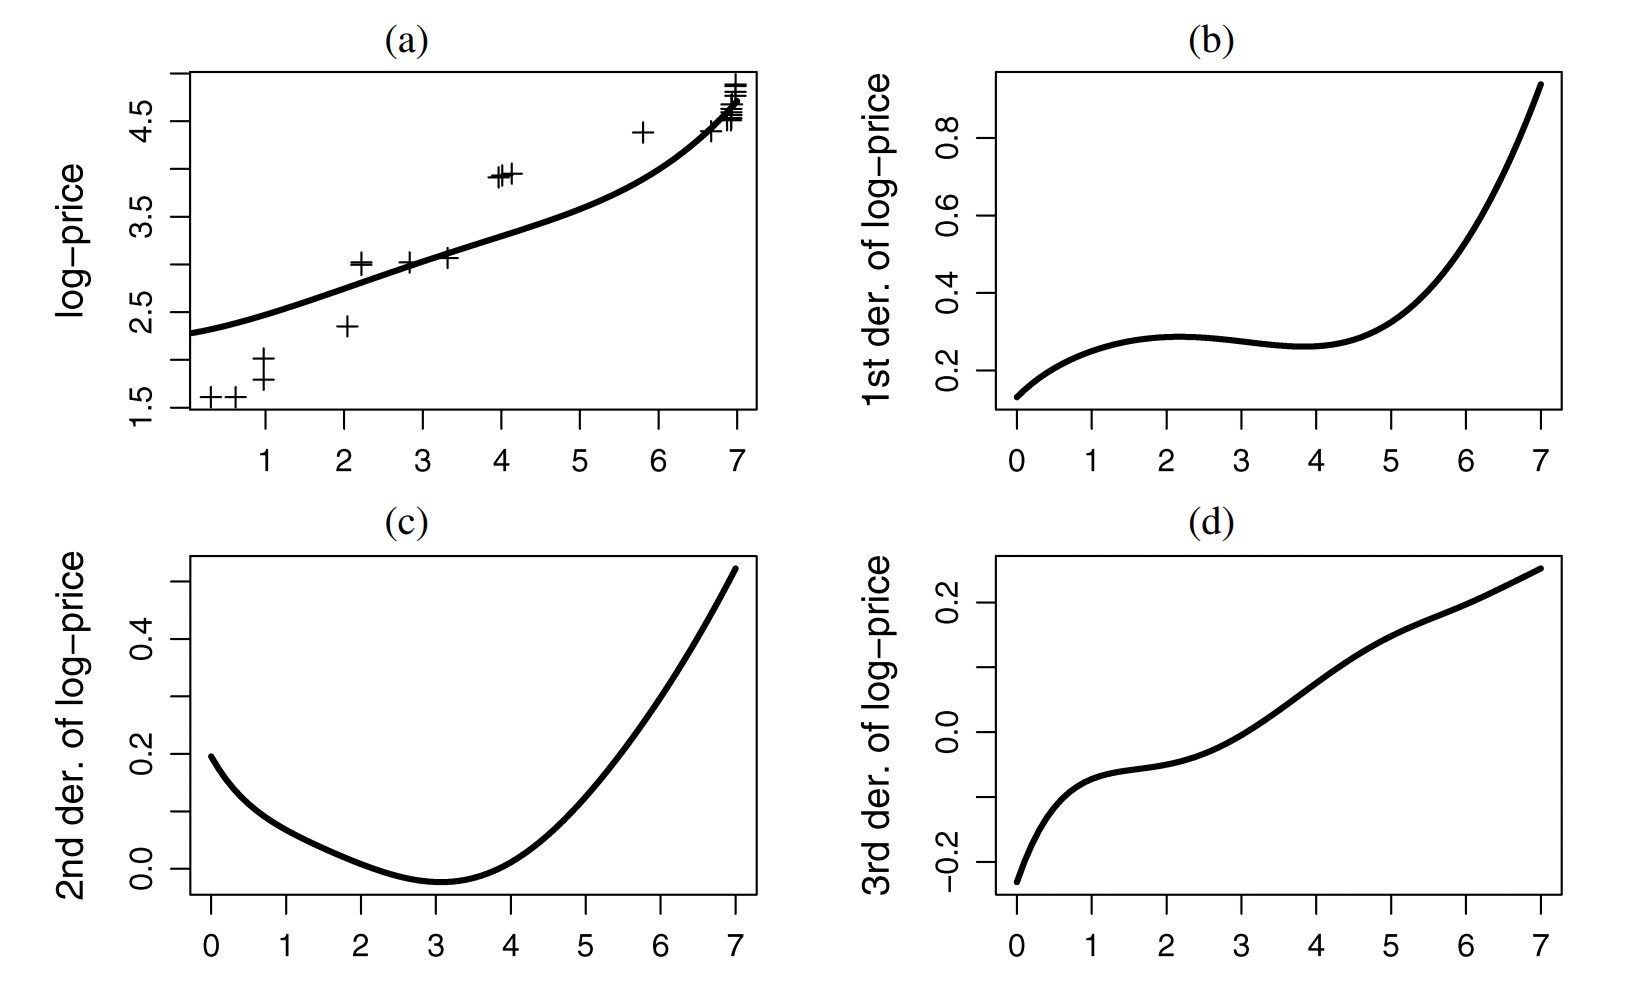
\includegraphics[width=1\textwidth]{smooth_velocity} %price increases monotonically, velocity stalls between 3 and 5
\end{frame}


\begin{frame}{Functional Regression Model} %time variyn variable amouunt of bids, time invariant reserve price, critic nothing said about epsilon
\begin{align}
\mathbf{y}(t) = [y_1(t),...,y_N(t)] \nonumber \\ \mathbf{X}(t)=\mathbf{X} \nonumber \\ \mathbf{y}(t)=\mathbf{X}^T\beta(t)+\mathbf{\epsilon}(t) \nonumber 
\end{align}
\end{frame}

\begin{frame}{Estimating the model}
\begin{itemize}
\item different approaches
\item fix a grid $t=t_1,...t_G$
\item for a fixed grid point, apply least squares
\item obtain estimates $\hat{\beta}(t_1),...,\hat{\beta}(t_G)$ 
\item smooth estimates to get functional estimate $\mathbf{\hat{\pmb{\beta}}}(t)$ 
\end{itemize}
\end{frame}

\begin{frame}{estimated parameter curves for price evolution} %muss interpretation zu jedem bild kennen nicht nur das was ich sagen will falls zb frage kommt % die variablen die ich in data erkläre hier interpretation zeigen!!!  computed confidence limits with +-2 standart errors
\center
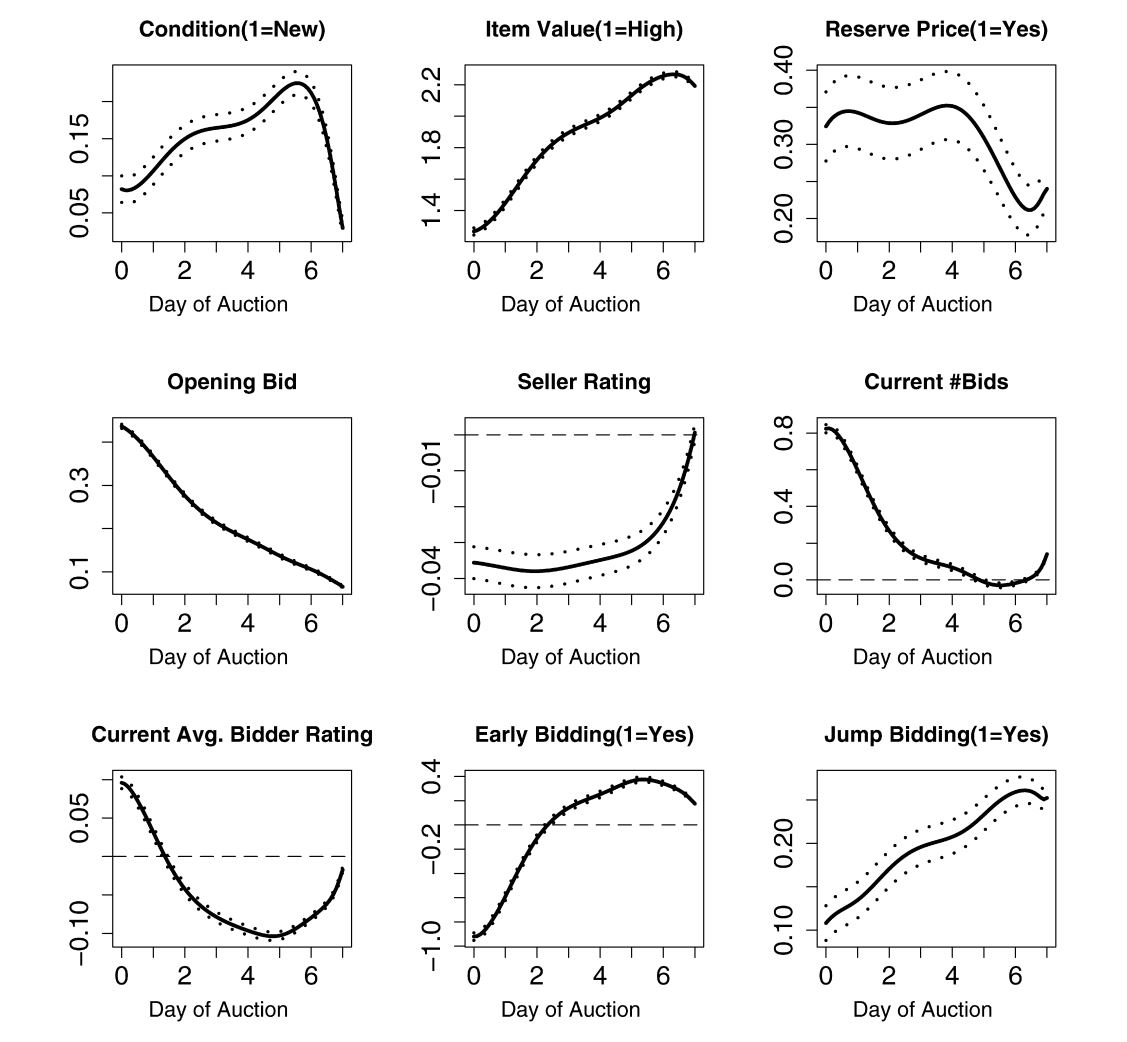
\includegraphics[width=0.7\textwidth]{price_evolution}
\end{frame}

\begin{frame}{estimated paramteter curves for price velocity}
\center
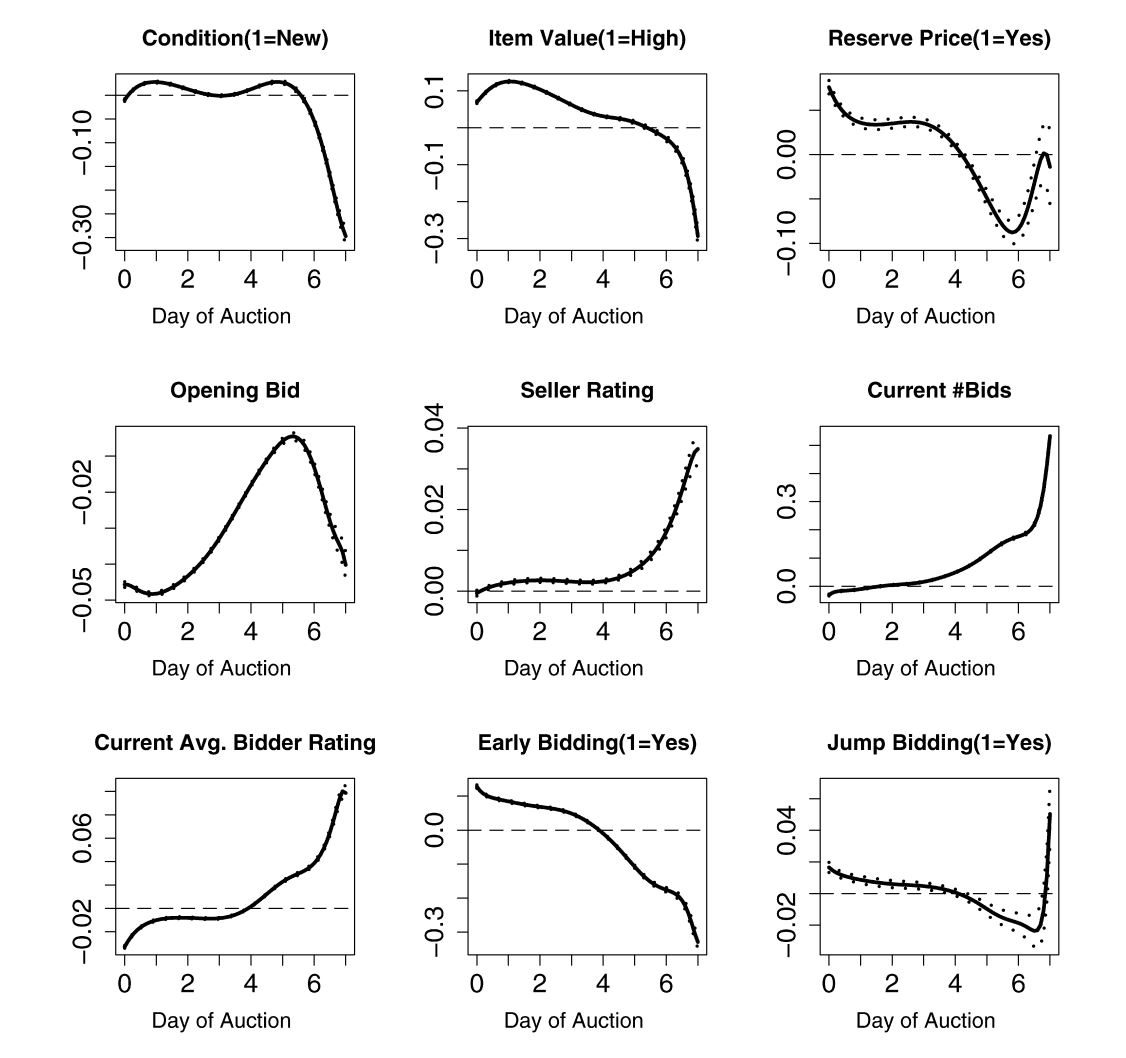
\includegraphics[width=0.7\textwidth]{price_velocity} % resrv price am ende weit auseindaner bounds weil durch smoorthing schlecht schätzbar eher nicht
\end{frame} %at any time opening bid and reserve price assosiated with higher price well known, not known before that  this holds during the whole auction,negative effect towrds end, opening bid positive effect on priceall the time but effect decreases, reason at hte beging not muczh information available except for opening bid but this changes over time, deriv always negative espacaly at the start and end, depress rate of price increase, puses bids closer to peoples cvaluation this decreases price dynamics, reserve price: assosicated with higher price but decreaes price dynamics seller rating: woukld thing actrs positivly but this is only the case  at the end of the auction,

\begin{frame}
\centering
The Dynamic Forecasting Model
\end{frame}

\begin{frame}{Dynamic forcasting model}
Four components
\begin{itemize}
	\item static predictor variables
	\item time-varying predictor variables
	\item price dynamics
	\item price lags
\end{itemize}	
\end{frame}

\begin{frame}{The model} %explain notation
\begin{equation}
y(t|t-1)=\alpha+\sum_{i=1}^{Q}\beta_ix_i(t)+\sum_{j=1}^J\gamma_jD^{(j)}y(t|t-1)+\sum_{l=1}^L\eta_ly(t-l|t-l-1) \nonumber
\end{equation}
\newline \\
\begin{itemize}
	\item $x_1,...x_Q$ is the set of static and time variying predictors
	\item $D^{(j)}y(t|t-1)$ is the jth derivative
	\item $y(t-l|t-l-1)$ price lags
\end{itemize}
\end{frame}

\begin{frame}{h-step-ahead prediction}
\small
\begin{equation}
\tilde{y}(T+h|T)=\hat{\alpha}+\sum_{i=1}^{Q}\hat{\beta}_ix_i(T+h|T)+\sum_{j=1}^J\hat{\gamma}_j\tilde{D}^{(j)}y(T+h|T)+\sum_{l=1}^L\hat{\eta}_l\tilde{y}(T+h-l|T) \nonumber
\end{equation}
\normalsize
\newline
Two challenges
\begin{itemize}
	\item at time $T \tilde{D}^{(j)}y(T+h|T)$ is not known
	\item static predictors in $x_i$ do not change over time
\end{itemize}
\end{frame}

\begin{frame}{forecasting price dynamics} %mind the notation! epsilon keine funktion 
We model $D^{(j)}y(t|t-1)$ as a polynomial in $t$ with autoregressive (AR) residuals
\begin{align}
D^{(j)}y(t|t-1) =\sum_{k=0}^Ka_kt^k+\sum_{i=1}^Pb_ix_i(t)+u(t) \ \ \ t=1,...,T \nonumber \\ \nonumber \\ u(t)=\sum_{i=1}^R\phi u(t-i)+\epsilon(t) \ \ \ \ \epsilon(t) \sim iidN(0,\sigma^2) \nonumber
\end{align} 
\end{frame}

\begin{frame}{forcasting price dynamics}
\begin{itemize}
	\item get estimates for all $a_k$, $b_i$ and $u(t)$
	\item use estimated residuals to estimate all $\phi_i$
	\item estimate next resdidual with \begin{equation}  \tilde{u}(T+1|T)=\sum_{i=1}^R\tilde{\phi}_iu(T-i+1) \nonumber \end{equation}
	\item lastly estimate the price derivative \begin{equation} D^{(j)}\tilde{y}(T+1|T) =\sum_{k=0}^K\hat{a}_k(T+1)^k+\sum_{i=1}^P\hat{b}_ix_i(T+1|T)+\tilde{u}(T+1|T) \nonumber \end{equation}
\end{itemize}	
\end{frame}

\begin{frame}{integrating static auction infromation}%opening bid has influence on price but this influnce vanishes over time
\begin{itemize}
	\item problem uncommon in time series analysis
	\item opening bid
	\item discounting
	\item $\tilde{x}(t)=x\tilde{\beta}(t)$
\end{itemize}
\end{frame}

\begin{frame}{Algorithm Outline}

\end{frame}

\end{document}